\section{Implémentation}

L'implémentation s'est fait au moyen de Matlab et des solveurs \texttt{quadprog} pour la génération de trajectoire et \texttt{fmincon} pour l'optimisation des temps de trajectoire. Pour commencer nous avons reproduit les résultats de Mellinger en faisait une trajectoire simple à travers les points $(0,0)$, $(1,0)$, $(1,2)$ et $(0,2)$ avec une allocation de temps égale à chaque segment de trajectoire et aucune contrainte sur les derivées, outre celles de continuité.

\begin{figure}[h]
\centering
\begin{subfigure}{.5\textwidth}
  \centering
  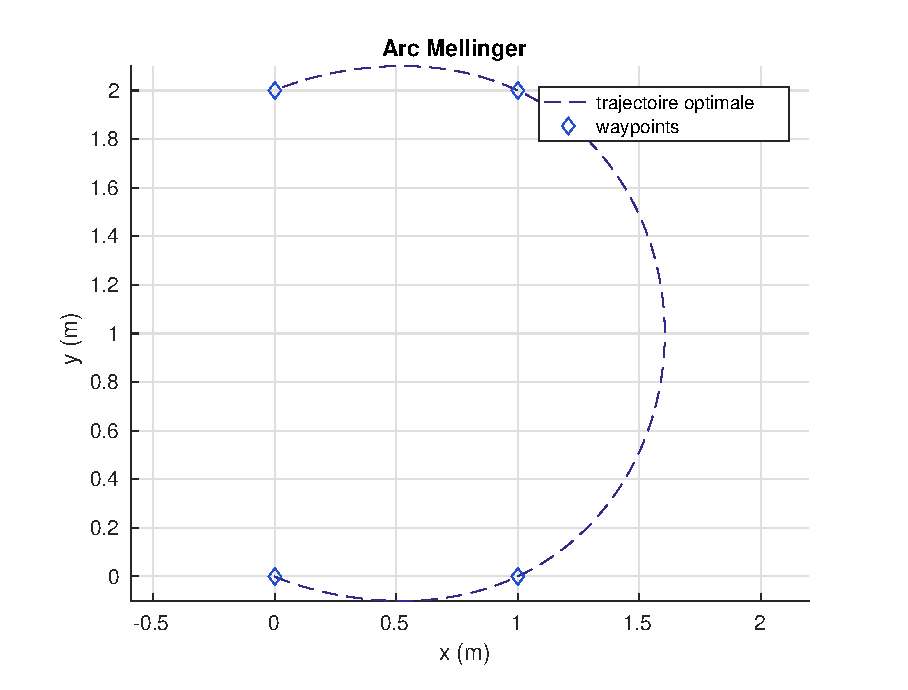
\includegraphics[width=\textwidth]{fig/arc_mellinger}
  \caption{Notre résultat}
\end{subfigure}%
\begin{subfigure}{.5\textwidth}
  \centering
  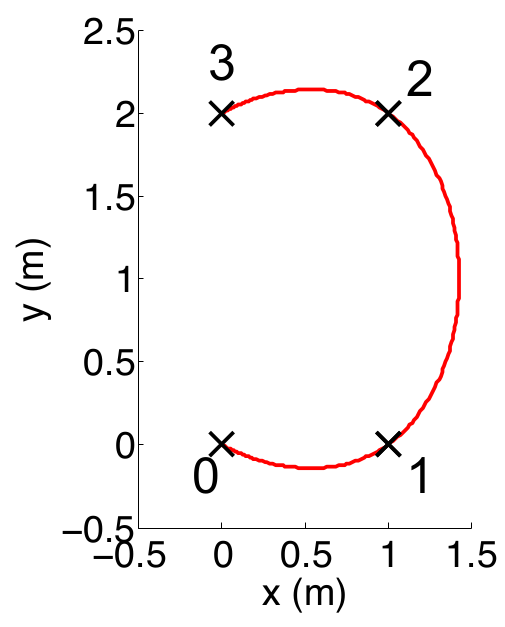
\includegraphics[width=0.6\textwidth]{fig/arc_mellinger_orig.png}
  \caption{Résultat de Mellinger \cite{Mellinger2011}}
  \label{fig:sub2}
\end{subfigure}
\caption{Comparaison de résultats}
\label{fig:comparaison}
\end{figure}

Nous voyons dans la figure (\ref{fig:comparaison}) que nous obtenons presque les mêmes résultats que dans \cite{Mellinger2011}. La différence entre les deux solutions pourrait  être reliée aux paramètres d'optimisation de \texttt{quadprog} ou les paramètres de tolérance sur la solution.

\begin{figure}[h]
\centering
\begin{subfigure}{.5\textwidth}
  \centering
  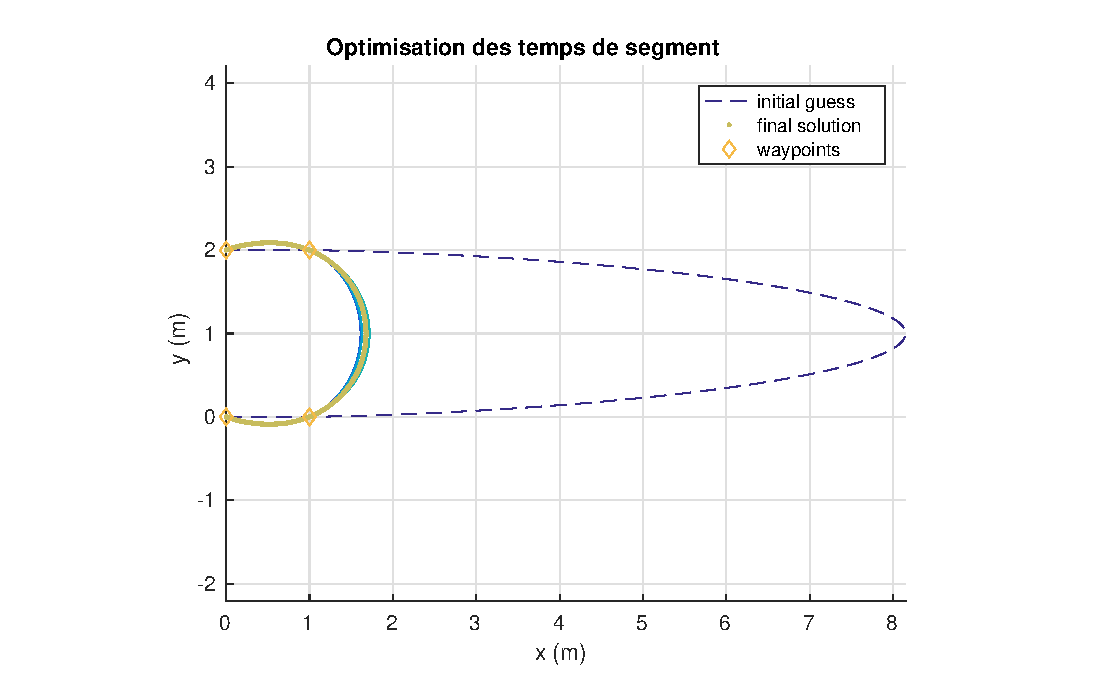
\includegraphics[width=1.2\textwidth]{fig/arc_time_opt}
  \caption{Résultat des itérations, l'allocation de temps initiale donnait beaucoup trop de temps au segment du milieu.}
\end{subfigure}%
\begin{subfigure}{.5\textwidth}
  \centering
  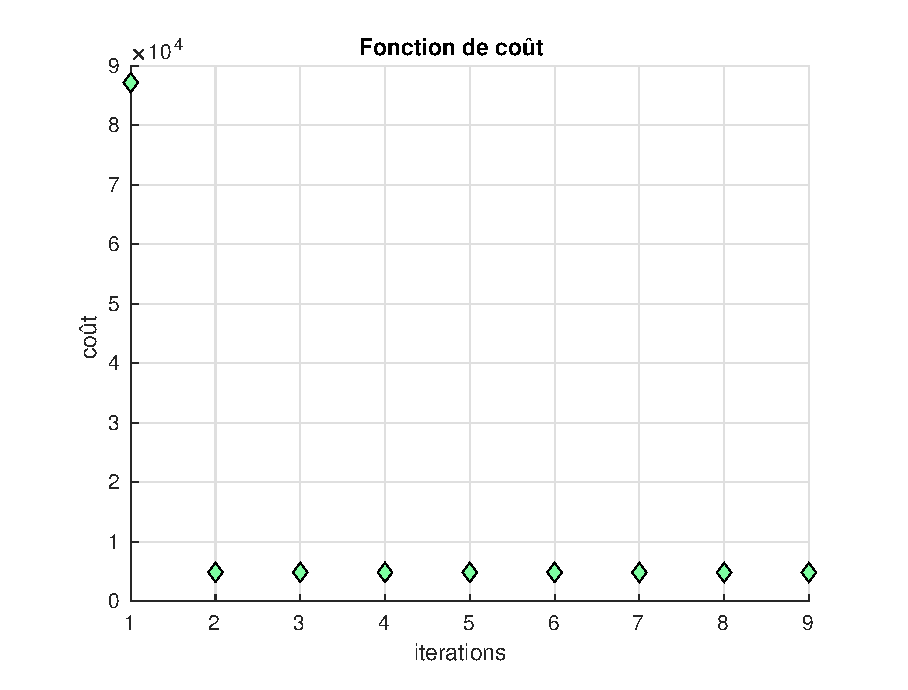
\includegraphics[width=\textwidth]{fig/cost}
  \caption{Valeur de la fonction de coût à chaque itération}
  \label{fig:sub2}
\end{subfigure}
\caption{Comparaison de résultats d'optimisation des temps de segment}
\label{fig:comparaison_opt_temps}
\end{figure}


Dans la figure (\ref{fig:comparaison_opt_temps}) nous voyons le résultat de l'optimisation des segments de temps. Notre méthode converge beaucoup plus rapidement que celle de Mellinger mais dans le même nombre d'itérations la raison n'est pas claire mais nous supposons que cela a rapport avec la valeur de $h$ utilisé pour calculer la dérivée et le choix de solveur et de ses paramètres. Mellinger ne spécifie pas le solveur qu'il a utilisé. Nous voyons aussi dans le bloc suivant la sortie de console de Matlab lors de l'optimisation.

\begin{verbatim}
>> main_optimt
                                            First-order      Norm of
 Iter F-count            f(x)  Feasibility   optimality         step
    0       1    8.711304e+04    0.000e+00    5.069e+05
    1       3    4.893364e+03    4.166e-12    3.105e+05    1.219e+00
    2       4    4.888882e+03    0.000e+00    3.882e+03    4.061e-03
    3       9    4.879789e+03    4.441e-16    1.242e+03    8.132e-03
    4      13    4.879264e+03    4.441e-16    1.193e+03    4.046e-03
    5      17    4.874708e+03    0.000e+00    1.210e+03    6.915e-02
    6      18    4.860743e+03    0.000e+00    4.416e+01    3.115e-02
    7      19    4.860729e+03    0.000e+00    3.209e+00    5.396e-04

Optimization stopped because the relative changes in all elements of x are
less than options.StepTolerance = 1.000000e-10, and the relative maximum constraint
violation, 0.000000e+00, is less than options.ConstraintTolerance = 1.000000e-06.

Optimization Metric                                           Options
max(abs(delta_x./x)) =   6.25e-11                       StepTolerance =   1e-10 (default)
relative max(constraint violation) =   0.00e+00   ConstraintTolerance =   1e-06 (default)

Elapsed time is 4.171527 seconds.
\end{verbatim}

Nous voyons que le processus prend étonamment longtemps ($4.17$ secondes) quoi que le tout a été calculé sur un vieux laptop avec beaucoup d'applications ouvertes.

Finalement, pour démontrer le fonctionnement de notre application dans toutes les dimensions, nous générons une trajectoire en slalom contenant aussi des variations en altitude.
\begin{figure}[h]
	\begin{center}
		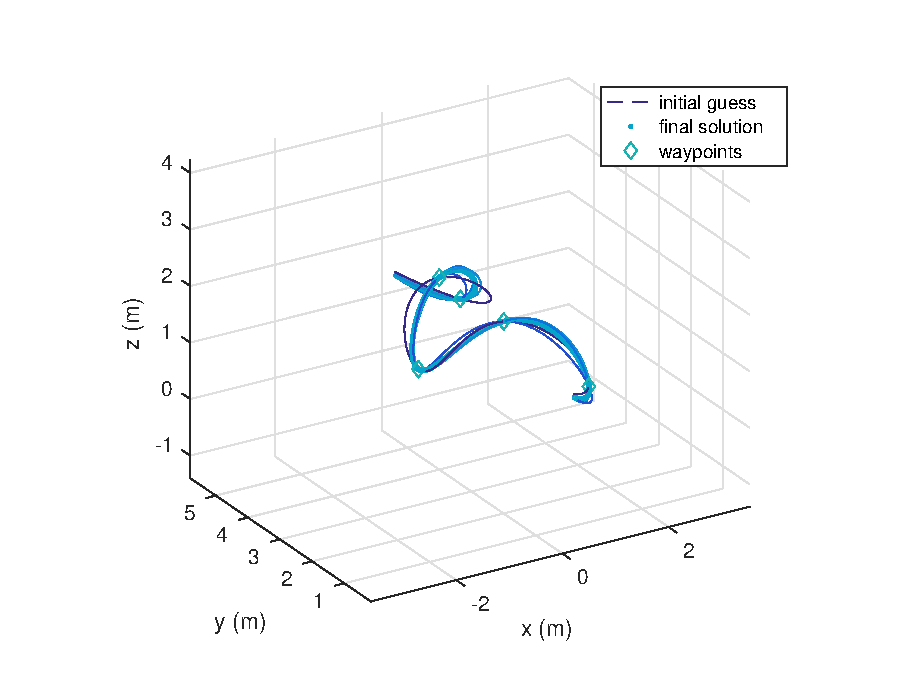
\includegraphics[width=0.5\textwidth]{fig/slalom}
		\caption{Slalom en 3 dimensions}	
	\end{center}
\end{figure}
